\section{Method}
\subsection{The experimental setup}

The experimental setup used to optically characterize the Fano mirrors, single- and double Fano cavities is illustrated in figure \ref{fig:experimental_setup} where the whole setup is sketched in figure \ref{fig:setup_sketch} and the specific part of the setup surrounding the cavity, outlined by the dashed line in figure \ref{fig:setup_sketch}, is subsequently shown in figure \ref{fig:setup_zoomed}. 

In order to effectively conduct the experiments in this project, it is imperative to be able to control certain parameters. Each element in the experimental setup is thoroughly considered for each their purpose in this regard, these will be outlined in this section. 

\begin{figure}[h!]
    \centering
    \begin{subfigure}[b]{0.4\textwidth}
        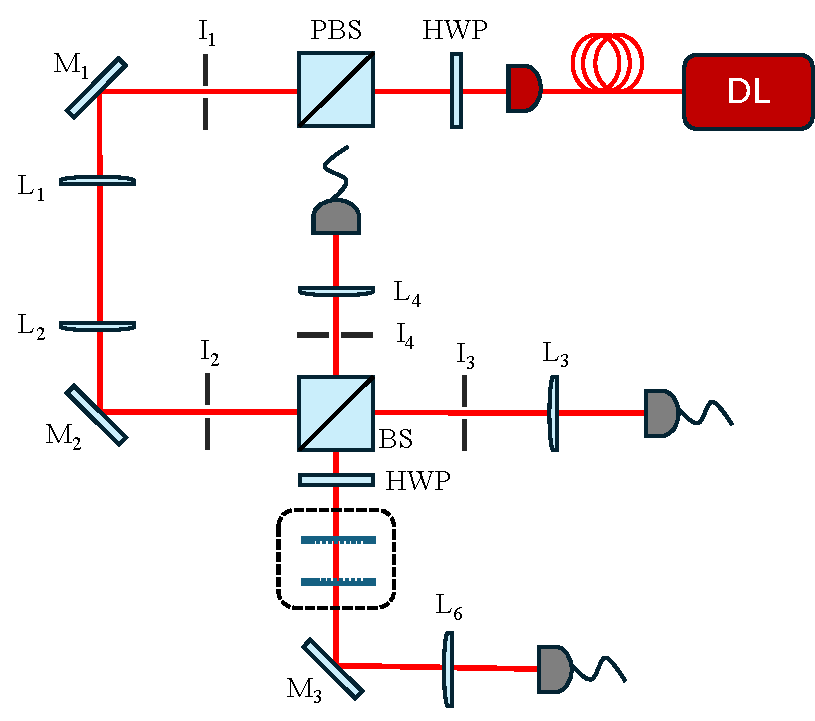
\includegraphics[width=\textwidth]{figures/setup_sketch.pdf}
        \caption{}
        \label{fig:setup_sketch}
    \end{subfigure}
    \hfill
    \begin{subfigure}[b]{0.59\textwidth}
        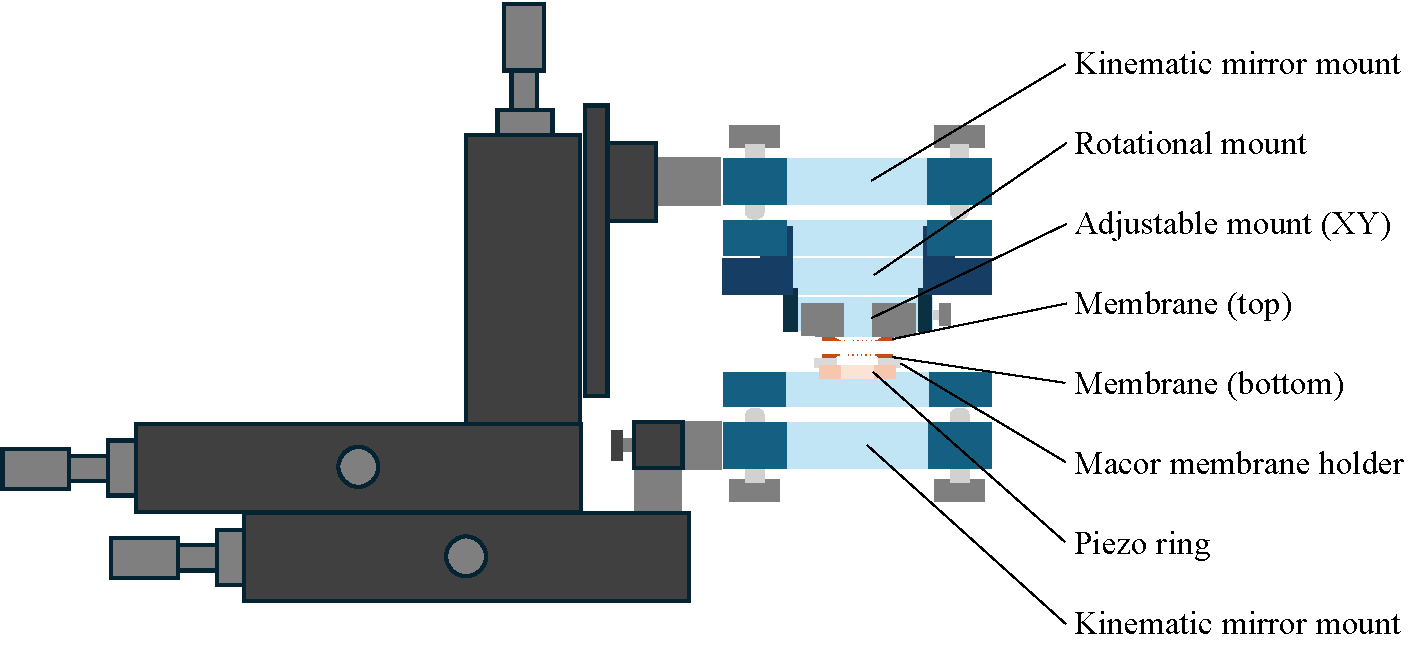
\includegraphics[width=\textwidth]{figures/setup_skecth_zoomed.pdf}
        \caption{}
        \label{fig:setup_zoomed}
    \end{subfigure}
    \caption{(a) shows schematics of the experimental setup for measuring cavity transmission- and Fano mirrors transmission/reflectivity spectra. The dashed line indicate the location of the cavity for measurements, and the setup is seen in (b). Note, the setup is shown with an optical cavity present, and is thus modified accordingly when prepared for Fano mirror measurements. The components not outlined in this section are regular mirrors labeled $M_{1-3}$ apatures used for alignment labeled $I_{1-4}$.}
    \label{fig:experimental_setup}
\end{figure}

\subsubsection{Tunable diode laser}

As shown in figure \ref{fig:experimental_setup} the laser source used for the optical characterizations is coupled into the setup through an optical fiber. The laser used is a \emph{Toptica DLC Pro} tunable CW diode laser with a range for the transmission wavelength of $910$ $-$ $980nm$. The optical fiber is a \emph{P3-780PM-FC-10} fiber from Thorlabs which is a single mode\footnote{A single mode fiber can only sustain the TEM00 mode, which means that the output is known to be perfectly Gaussian.} polarization-maintaining optical fiber with an effective range of $770$ $-$ $1100nm$. Between the Toptica laser and the incoupling end of the fiber, a $\lambda/2$\emph{-plate} (HWP) and \emph{polarizing beam splitter} (PBS) is placed in order to be able to control the incident power of the laser and to only couple linearly polarized light into the setup.  

The light being emitted from the optical fiber is sent through another HWP and PBS in order to be able to control the resulting polarization in the setup even more precisely, should there be any discrepancies of the light coupled into the fiber. 

\subsubsection{$\lambda / 2$ - waveplate}

A $\lambda/2$-waveplate, or HWP, is constructed of a so-called bi-refringent material (most commonly crystaline quartz), which means that it has slightly different refractive indicies for incident light of different polarization axis'. Generally a HWP will have a \emph{fast}- and \emph{slow axis}, where it is understood that light polarized along the fast axis experiences a lower refractive index (and hence moves faster), than that along the slow axis. In this way the HWP separates the components of unpolarized light that has perpendicular and parallel polarizations with respect to the fast axis. 

\begin{figure}[h!]
    \centering
    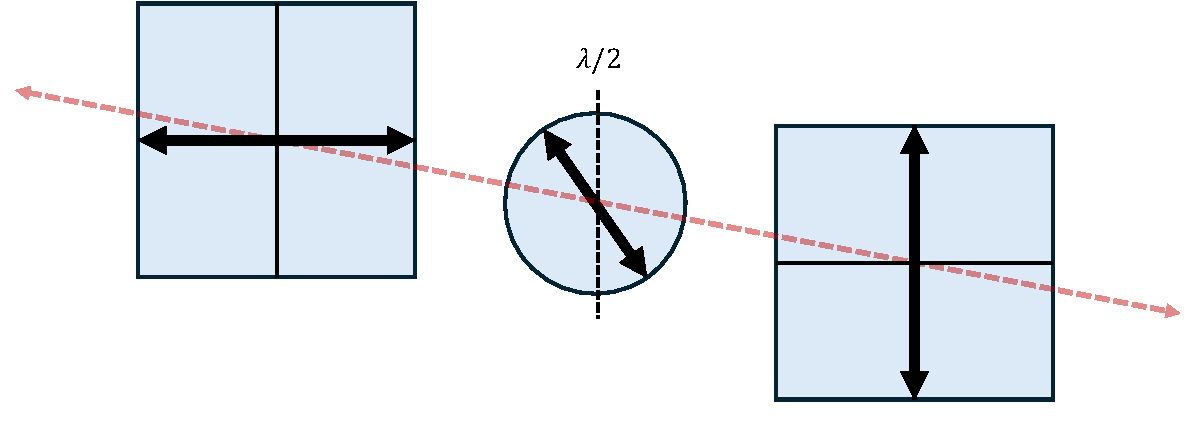
\includegraphics[width=0.6\textwidth]{figures/HWP.pdf}
    \caption{A simple sketch of the effect of a HWP on linearly polarized light.}
    \label{fig:HWP}
\end{figure}

The effect of the HWP on linearly polarized light, is an effective rotation of the polarization, this is sketched simply in figure \ref{fig:HWP}. It can be shown that the polarization axis is rotated according to the angle between the fast axis of the HWP and the incident polarization axis. A relative angle $\theta$ will thus result in a rotation of $2\theta$, e.g. if $\theta=45^{\circ}$, this will constitute a rotation from completely p-polarized light to completely s-polarized light. This is the specific scenario sketched in figure \ref{fig:HWP}\cite{edmund_optics}. In this way a rotating HWP can allow one to alter an incident linearly polarized beam to be polarized along any axis, and is thus a necessary component for this particular setup.

\subsubsection{Optical telescope}

The linearly polarized light transmitted through the PBS passes through plano-convex lenses of positive focal lengths $f$ and $f^{\prime}$, $L_1$ and $L_2$, which together makes up an optical telescope used to manipulate the beam waist $w_0$ incident on the cavity or Fano mirror. 

Figure \ref{fig:telescope} shows schematics of the general way an optical telescope is utilized to manipulate the beam waist of a laser beam.

\begin{figure}[h!]
    \centering
    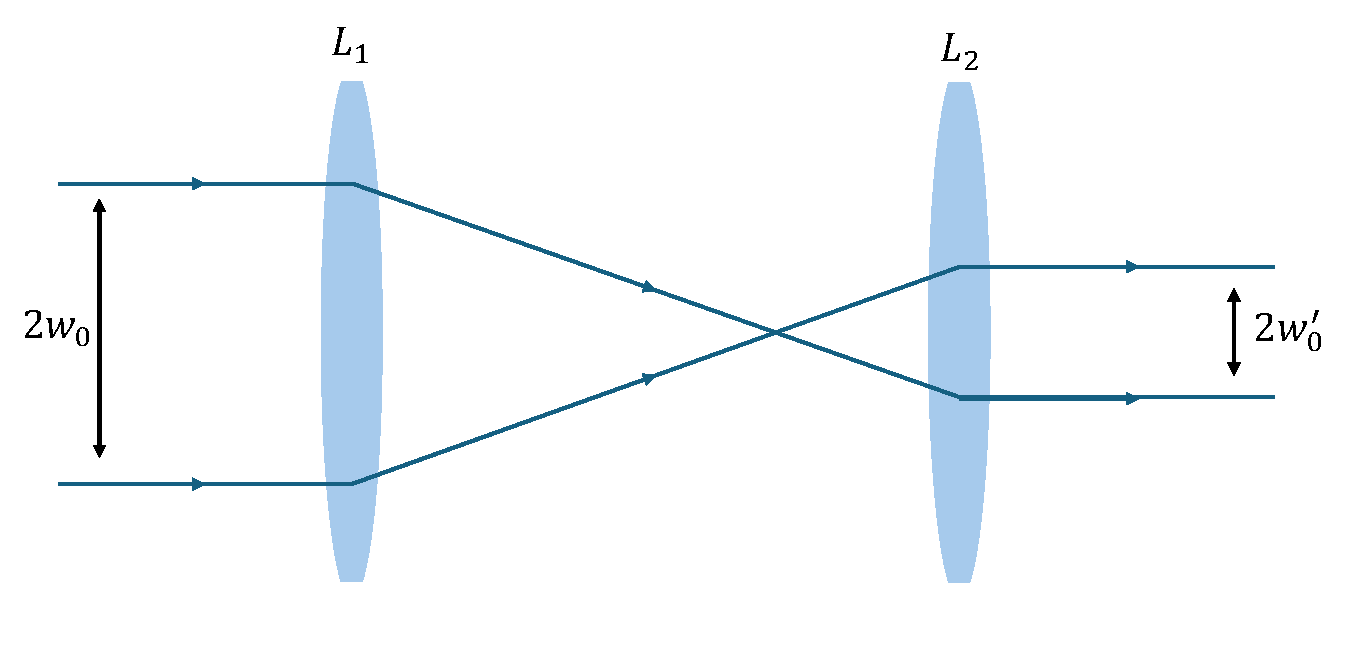
\includegraphics[width=0.5\textwidth]{figures/optical_telescope.pdf}
    \caption{}
    \label{fig:telescope}
\end{figure}

When the incident beam hits $L_1$ it is focused according to its focal length $f$, and by inserting another lens $L_2$ of a relatively longer focal length one can \emph{catch} the beam at the desired beam waist. If the focal length $f^{\prime}$ of $L_2$ is sufficently long, compared to the path of the beam after the lenses, the beam will be approximately collimated and remain at the waist obtained when incident on $L_2$.

\subsubsection{Transmission, reflection and incident photo-detectors}

After passing the optical telescope the beam reaches a simple 50/50 beam splitter (BS) which transmits 50\% of the light while reflecting another 50\%. The reflected light is then incident on the cavity or Fano mirror (target). 

The transmitted light passes through a lens $L_3$, which is focused on a photo-detector $P_I$ used for reference measurements and later normalization. Since the tunable laser in nature varies in power with the wavelength, it is necesarry to keep track of these fluctuations and correct for them in data analysis. 

The transmitted light is sent through, yet another, HWP which in this case is used only to alter the polarization of the light incident on the target. After the beam, or a portion of it, has passed the target it is sent through a lens $L_5$ focused onto the transmission detector $P_T$.

The part of the light incident on the target that is \emph{not} transmitted, is reflected back onto the BS which then transmits 50\% once again, and thus reflects the other 50\%. The transmitted part here is focused through the lens $L_4$ onto the reflection detector $P_R$.

\subsubsection{The double Fano cavity measurement setup}

The cavity measurement setup shown in figure \ref{fig:setup_zoomed} is the one used to measure the transmission spectrum of a double Fano cavity consisting of two Fano mirrors. This part of the setup consists of two sets of standard \emph{PT1} $\mu m$-stages from Thorlabs combined to provide precise movement of each Fano mirror in the xy-plane. 

\begin{figure}[h!]
    \centering
    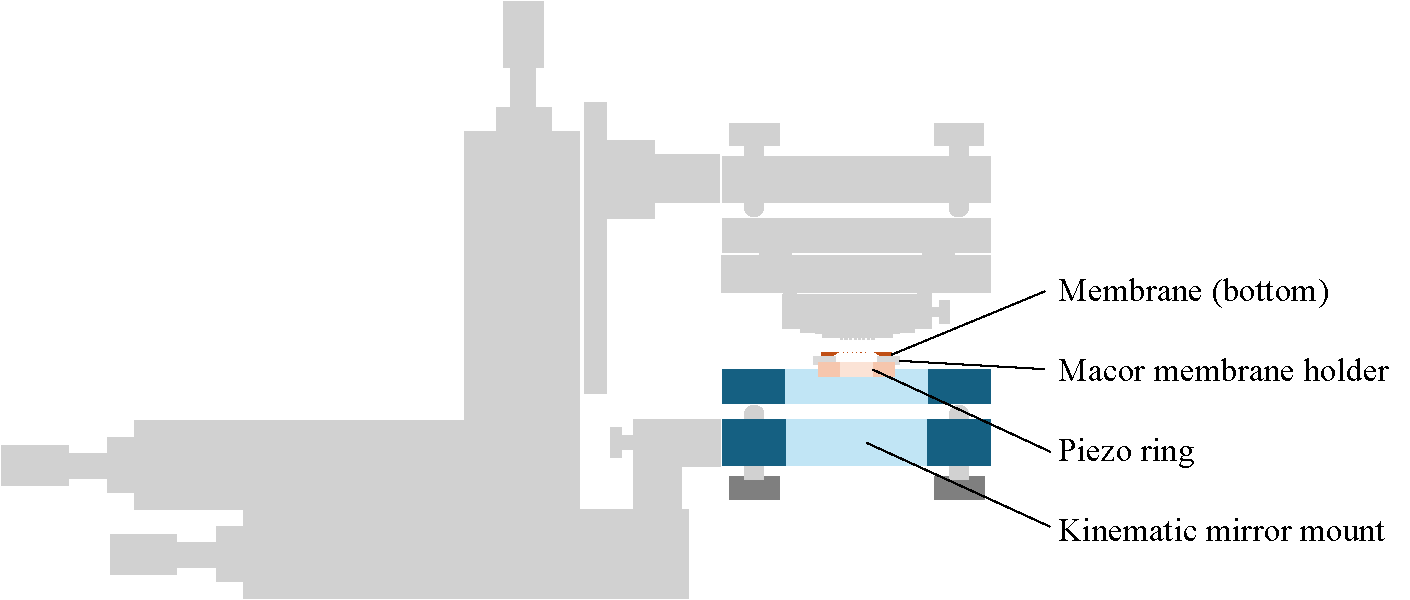
\includegraphics[width=0.6\textwidth]{figures/setup_bottom.pdf}
    \caption{Schematics of the \emph{bottom} part of the double Fano cavity setup.}
    \label{fig:setup_bottom}
\end{figure}

Examining the structure from the bottom (as it is built), a kinematic mirror mount is attached to the lower set of xy-stages, this is used to control the angular degrees of freedom of the Fano mirror which makes up the bottom of the cavity. On the mirror mount, a piezo ring is firmly attached and connected to a piezo driver and that to a function generater in order to control the expansion of the piezo ring both by application alternating and fixed current. Lastly, in order to be able to place the Fano mirror or simply membrane on the  piezo ring, a ceramic Macor membrane holder is used. The bottom part of the cavity setup is highlighted in figure \ref{fig:setup_bottom}.

\begin{figure}[h!]
    \centering
    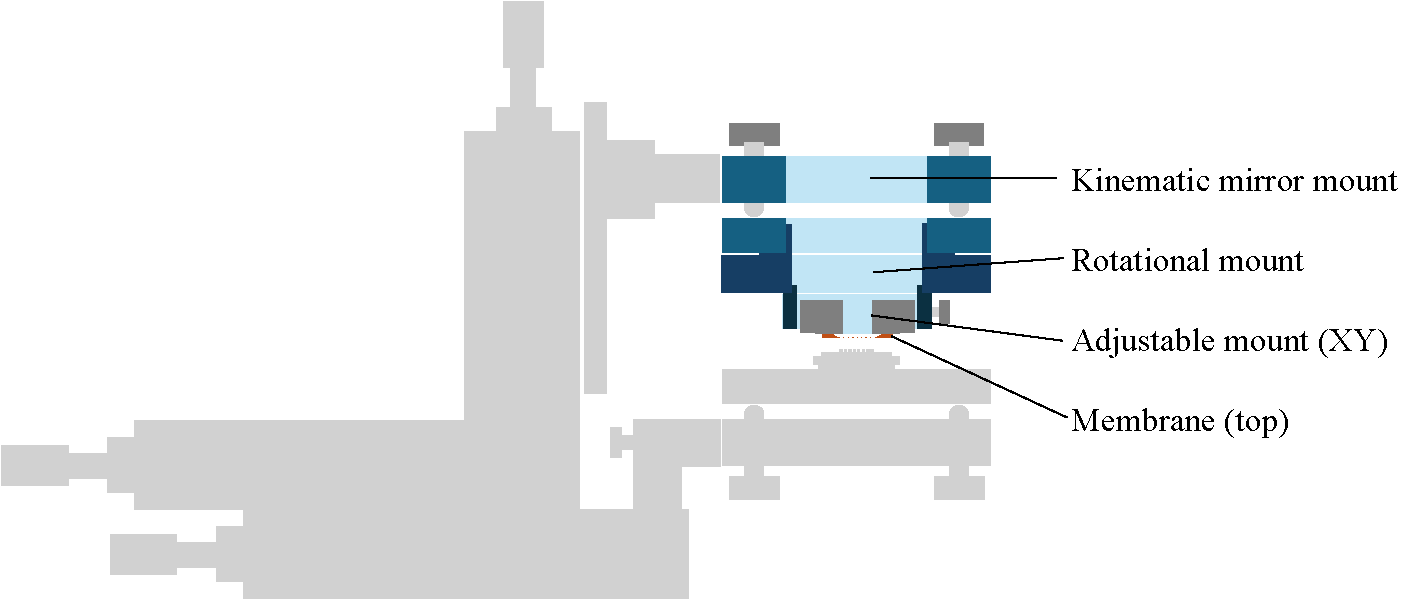
\includegraphics[width=0.6\textwidth]{figures/setup_top.pdf}
    \caption{Schematics of the \emph{top} part of the double Fano cavity setup.}
    \label{fig:setup_top}
\end{figure}

The part of the setup built to control the Fano mirror making up the top of the cavity is slightly more complicated, as this is the Fano mirror that is, for practical reasons, aligned last. This means that additional degrees of freedom must be controled by movement of the Fano mirror itself. The alignment procedure will be explained in detail in sections \ref{sec:grating_characterization} and \ref{sec:cavity_measurements}. 

The top part of the cavity setup is attached to the second set of xy-stages and additionally to an \emph{NFL5DP20} stage from Thorlabs in the z-direction in order to be able to change the length of the cavity. As for the bottom part of the cavity setup, a kinematic mirror mount acts as the base of the construction. This is, once again, to control the angular degrees of freedom of the corresponding Fano mirror. On the mirror mount, a standard rotational mount with a 1 inch inner winding is attached in order to be able to control the rotational degree of freedom of the Fano mirror. An additional xy-adjustable mount is then used in order to effectively place the Fano mirror in the center of the rotational mount to ensure the rotational axis is in the center of the membrane. Finally, the Fano mirror is taped to a costume mount created to fit into the xy-adjustable mount. The top part of the cavity setup is highlighted in figure \ref{fig:setup_top}.

What has been outlined here is the setup utilized to optically characterize the double Fano cavity. If one wishes to do so for the single Fano cavity instead, the setup would be modified such that the top part of the setup, highlighted in figure \ref{fig:setup_top}, would only consist of the kinematic mirror mount. Inside the mirror mount would then be placed a broadband mirror. The rotational- and xy-adjustable mounts would here be redundant due to the rotational symmetry of any standard broadband mirror.
